%where the control of external atmospheric conditions is less accurate

The measurements obtained with the TRITIUM-Aveiro prototype in the Arrocampo dam are reported in this section. This prototype recorded data for more than four months (27/03/2019 to 18/08/2019). The data acquired during this time are plotted in Figure \ref{fig:BackgroundArrocampoAveiro}, for bins of 60 minutes.
\begin{figure}[h]
\centering
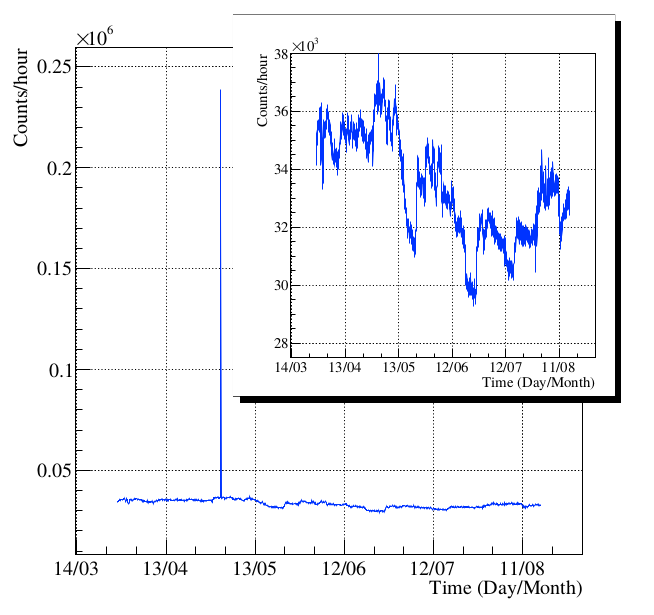
\includegraphics[scale=0.6]{5Prototypes/54ArrocampoMeasurements/721TRITIUMAVEIRO0/BackgroundMeasurements.png}
\caption{Background measured with TRITIUM-Aveiro in the Arrocampo site \cite{ExperimentalPaperCarlos}.\label{fig:BackgroundArrocampoAveiro}}
\end{figure}
The data look stable during the measuring period. An average rate of $9.3~\second^{-1}$ was obtained. A narrow peak is observed on May 2 caused by the removal of part of the lead shield top for an intervention in the prototype. The data are magnified in the inset of the figure. The MDA measured in the Arrocampo dam for a $60~\min$ integration time is 6 times larger than in the laboratory measurements (section \ref{subsec:TritiumAveiro}). This may be due to the electric noise introduced by the pumps of the water purification system and the instability observed in the electronic boards.

%The cosmic veto currently under development is going to be installed in anti-coincidence with two additional prototypes. Furthermore, three TRITIUM-IFIC-2 prototypes and a cosmic veto are also planned to be installed in the Arrocampo site as soon as possible.